% !TeX root = ../main.tex
% Add the above to each chapter to make compiling the PDF easier in some editors.

\chapter{Electrical Flows}

A classical graph problem is the flow of electrical currents through a network of resistors. Such a network $G = (\sV, \sE, \vr)$ can be described by a set of vertices $\sV$, set of wires (or edges) $\sE$, and resistances $\vr \in \R_{>0}^{|\sE|}$ of wires. We are interested in finding the electrical flow $\vf \in \R^{|\sE|}$ through the network, assigning to each wire the current that is transported per unit time. Alternatively, we can think of voltages $\vx \in \R^{|\sV|}$ at the vertices, which Ohm's law relates to the electrical flow.

By \emph{Ohm's law}\index{Ohm's law}, we have that for any wire $e \in \sE$, \begin{align}
    \vf(e) = \frac{\vx(e)}{\vr(e)}, \quad \vx(e) = \vf(e) \cdot \vr(e),
\end{align} where $\vx(\{u,v\}) \defeq \vx(u) - \vx(v)$ is the voltage difference of vertices $u$ and $v$. The \emph{net flow}\index{net flow} of current at a vertex $u \in \sV$ is given as, \begin{align}
    \sum_{v \sim u} \vf(v, u).\margintag{We use $v \sim u$ to denote all $v$ that are adjacent to $u$.}
\end{align} We say that a flow routes \emph{demand}\index{demand} $\vd \in \R^{|\sV|}$ if the net flow at every vertex is $\vd(v)$. The fact that at vertices with zero demand, the flow is conserved\footnote{As much current is flowing into the vertex as is flowing out of it.} is also known as \emph{Kirchhoff's current law}\index{Kirchhoff's current law}.

\begin{marginfigure}
    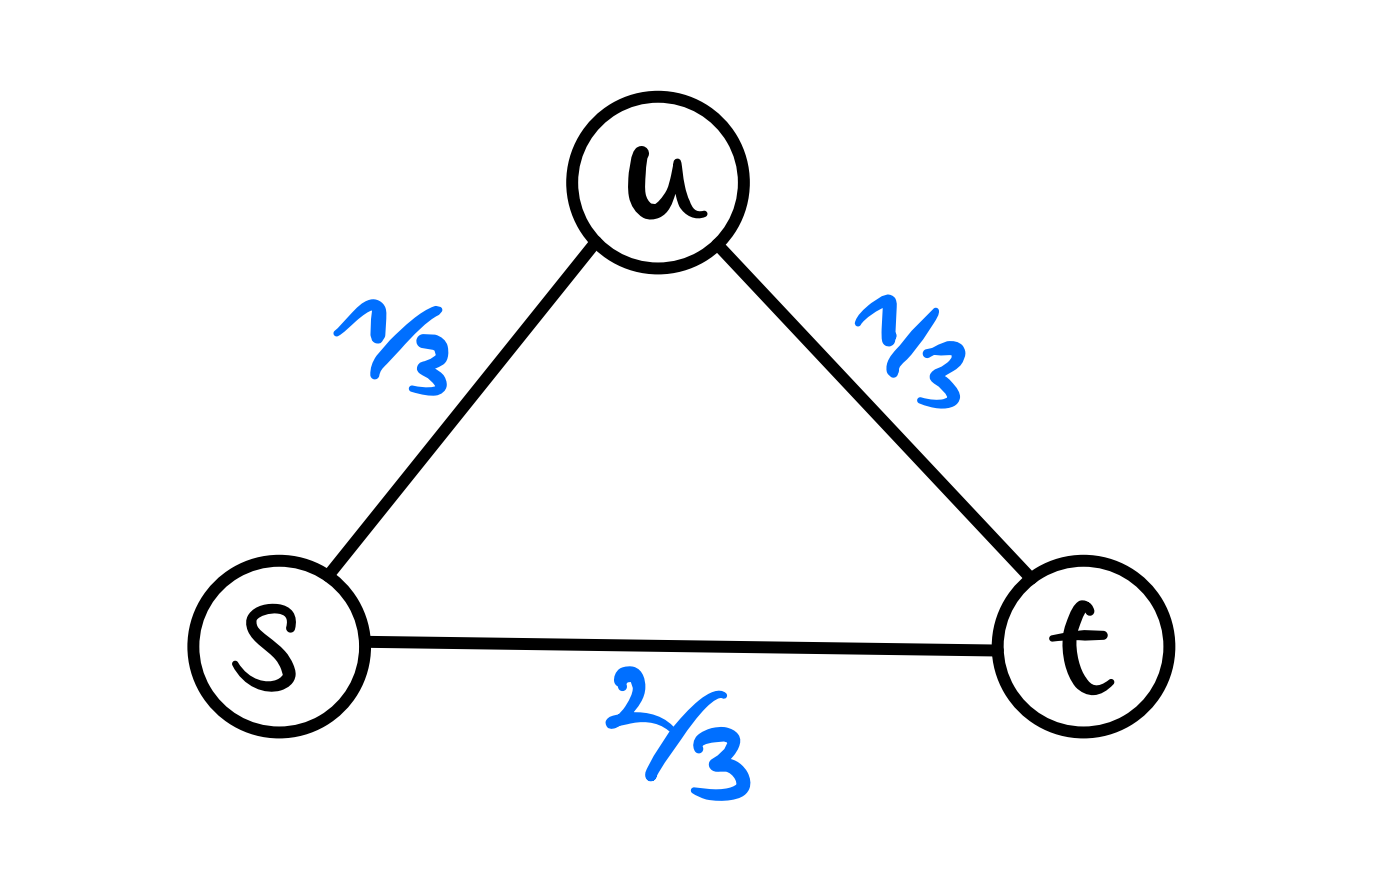
\includegraphics[width=\textwidth]{notes/figures/electrical_flows.png}
    \caption{Example of an electrical flow (shown in blue) with voltages \begin{align*}
        \vx(s) = 0,\quad \vx(u) = 1,\quad \vx(t) = 2
    \end{align*} and unit resistances, routing demands \begin{align*}
        \vd(s) = -1,\quad \vd(u) = 0,\quad \vd(t) = 1.
    \end{align*}}
\end{marginfigure}

To keep track of the direction of flow on each edge, we assign an arbitrary direction to each edge (we ``orient'' $G$) and only consider non-negative flows, $\vf \in \R_{\geq 0}^{|\sE|}$. Clearly, for any previously feasible flow, we can assign directions in such a way that the flow remains feasible.

\section{The Laplacian Matrix}

\begin{defn}[Adjacency matrix]\index{adjacency matrix}
The \emph{adjacency matrix} of a graph $G$, $\Tilde{\mA} \in \R^{|\sV|\times|\sV|}$, is defined as,\footnote{By $\mA$ we will later denote the weighted adjacency matrix.} \begin{align}
    \Tilde{\mA}(u, v) \defeq \begin{cases}
        1 & \text{if $u \sim v$} \\
        0 & \text{otherwise}.
    \end{cases}
\end{align}
\end{defn}
\begin{defn}[Incidence matrix]\index{incidence matrix}
The \emph{incidence matrix} of an oriented graph $G$, $\mB \in \R^{|\sV|\times|\sE|}$, is defined as, \begin{align}
    \mB(v, e) \defeq \begin{cases}
        1 & \text{if $e = (u,v)$ for some $u \in \sV$} \\
        -1 & \text{if $e = (v,u)$ for some $u \in \sV$} \\
        0 & \text{otherwise}.
    \end{cases}
\end{align}
\end{defn} Each column of $\mB$ only has two non-zero entries and sums to one.
\begin{marginfigure}
    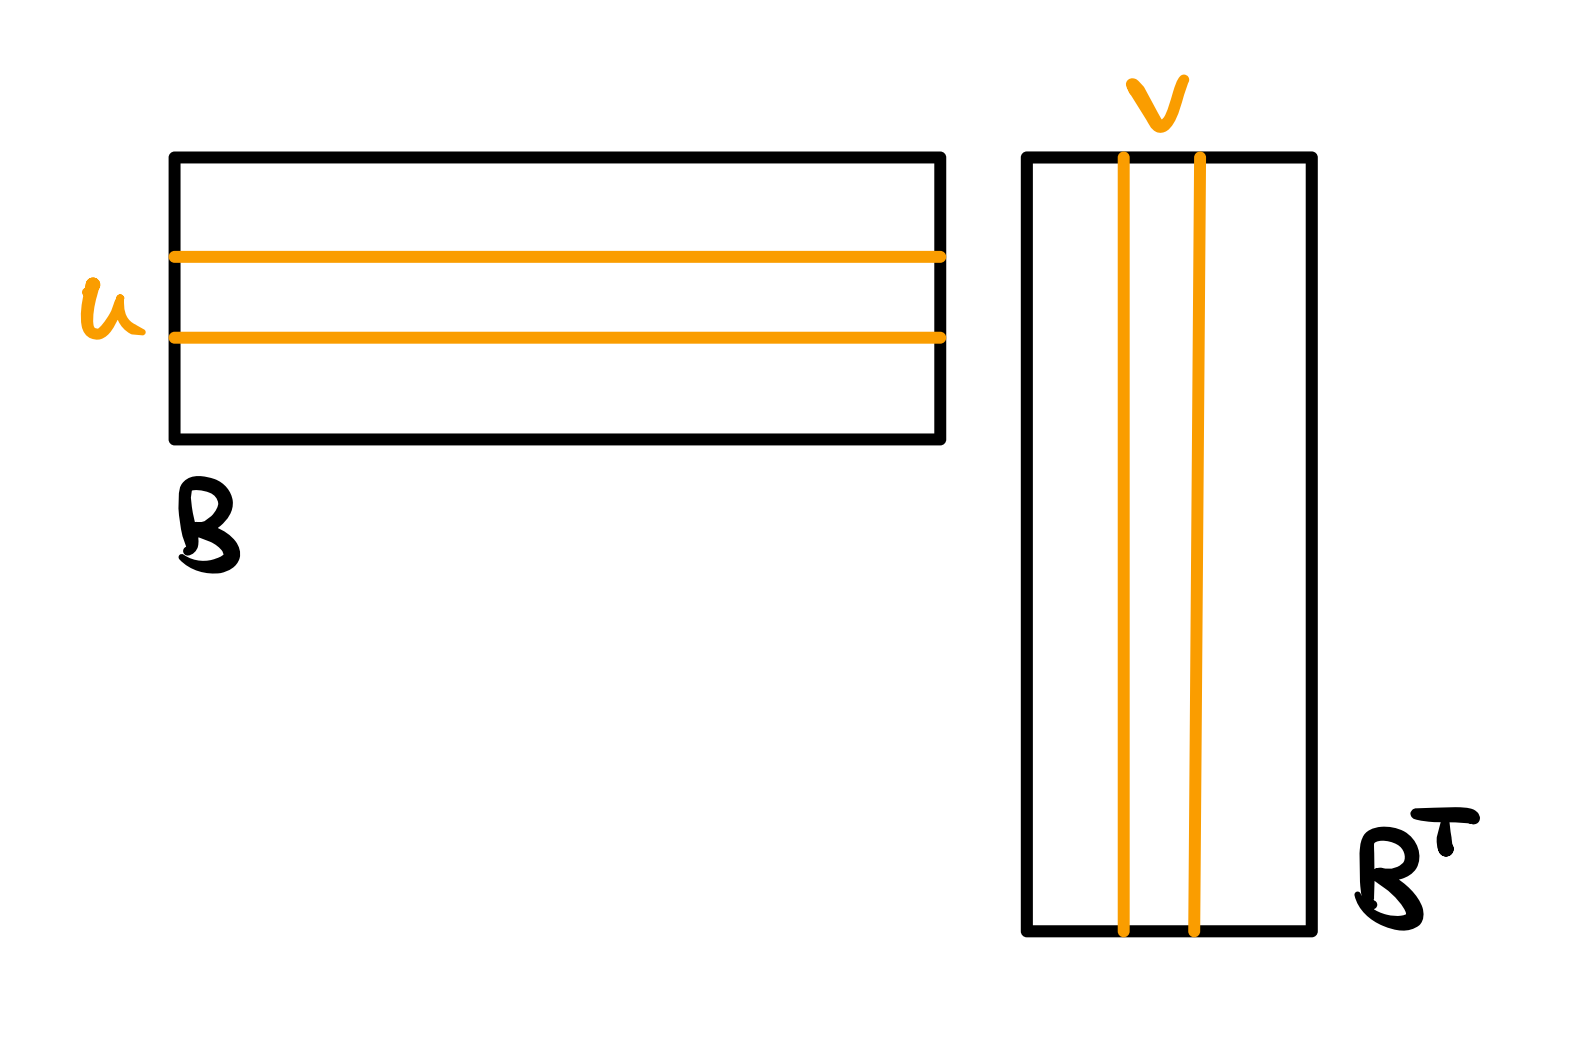
\includegraphics[width=\textwidth]{notes/figures/incidence_matrix.png}
    \caption{Illustration of the matrix product $\mB\trans{\mB}$.}
\end{marginfigure}
\begin{lem}\label{lem:incidence_matrix_product}
$\mB \trans{\mB} = \diag\{\deg(v)\}_{v \in \sV} - \Tilde{\mA}$.
\end{lem}
\begin{proof} The dot product of the rows, corresponding to the same vertex $v$, produces exactly $\deg(v)$. All other dot products between rows corresponding to vertices $u$ and $v$ are $-1$ iff $u \sim v$ and $0$ otherwise.
\end{proof}
We can now also write the net flow constraint\index{net flow constraint}, \begin{align}
    \mB\vf = \vd.
\end{align} We define $\mR \defeq \diag\{\vr(e)\}_{e \in \sE}$ and then have that Ohm's law\index{Ohm's law} can be expressed as, \begin{align}
    \trans{\mB}\vx = \mR\vf, \quad\text{or equivalently,}\quad \mR^{-1}\trans{\mB}\vx = \vf.
\end{align} If the net flow constraint is satisfied, this yields, \begin{align}
    \underbrace{\mB\mR^{-1}\trans{\mB}}_{\text{Laplacian}}\vx = \mB\vf = \vd. \label{eq:ohms_law_and_net_flow_constraint}
\end{align}
\begin{defn}[Laplacian matrix]\index{Laplacian matrix}\label{defn:laplacian_matrix}
The \emph{Laplacian matrix} of an oriented graph $G$ is defined as, \begin{align}
    \mL \defeq \mB\mR^{-1}\trans{\mB} = \mB\mW\trans{\mB} \in \R^{|\sV|\times|\sV|},
\end{align} where $\mW \defeq \mR^{-1}$ is a diagonal matrix of weights\index{weight (of an edge)} $\vw(e) \defeq \frac{1}{\vr(e)}$.
\end{defn}\noindent Intuitively, the weight of an edge can be understood as how ``connected'' the two vertices at its endpoints are. In contrast, the resistance of an edge is smaller when endpoints are well-connected.

We will now learn a little more about Laplacian matrices.
\begin{defn}[Weighted adjacency matrix]\index{weighted adjacency matrix}
The \emph{weighted adjacency matrix} of a graph $G$, $\mA \in \R^{|\sV|\times|\sV|}$, is defined as, \begin{align}
    \mA(u, v) \defeq \begin{cases}
        w(\{u,v\}) & \text{if $u \sim v$} \\
        0 & \text{otherwise}.
    \end{cases}
\end{align}
\end{defn}
\begin{lem}
$\mA$ is symmetric, that is, $\mA = \trans{\mA}$.
\end{lem}
\begin{proof}
This follows immediately from the fact that $G$ is undirected.
\end{proof}
\begin{defn}[Weighted degree]\index{weighted degree}
The \emph{weighted degree} of a vertex $v \in \sV$ is given as, \begin{align}
    \vd(v) \defeq \sum_{\{u,v\} \in \sE} \vw(\{u,v\}).
\end{align} We write $\mD \defeq \diag\{\vd(v)\}_{v \in \sV}$.
\end{defn}

\begin{lem}
$\mL = \mD - \mA$.
\end{lem}
\begin{proof}
The proof is identical to the proof of \cref{lem:incidence_matrix_product}, only that every entry is now weighted, due to the additional factor $\mW$.
\end{proof}

\begin{cor}
$\mL$ is symmetric.
\end{cor}
\begin{proof}
This directly follows from the fact that $\mD$ and $\mA$ are symmetric.\footnote{Diagonal matrices like $\mD$ are trivially symmetric.}
\end{proof}

\begin{lem}
For any $\vx \in \R^{|\sV|}$, we have, \begin{align}
    \trans{\vx}\mL\vx = \sum_{\{u,v\}\in\sE} \vw(\{u, v\})[\vx(u) - \vx(v)]^2 \geq 0. \label{eq:laplacian_quadratic_form}
\end{align}
\end{lem}
\begin{proof}
We have, \begin{align*}
    \trans{\vx}\mL\vx &= \trans{\vx}\mD\vx - \trans{\vx}\mA\vx. \\
    \trans{\vx}\mD\vx &= \sum_{v \in \sV} \vd(v) \vx(v)^2 = \sum_{\{u,v\}\in\sE} \vw(\{u,v\})[\vx(u)^2 + \vx(v)^2]. \\
    \trans{\vx}\mA\vx &= \sum_{v \in \sV} \vx(v) (\mA\vx)(v) \\
    &= \sum_{v \in \sV} \vx(v) \sum_{u \in \sV} \mA(v,u) \vx(u) \\
    &= \sum_{v,u \in \sV} \vw(\{u,v\})\vx(u)\vx(v) \\
    &= 2 \sum_{\{u,v\}\in\sE} \vw(\{u,v\})\vx(u)\vx(v).
\end{align*} Combining the above equalities, we obtain, \begin{align*}
    \trans{\vx}\mL\vx &= \sum_{\{u,v\}\in\sE} \vw(\{u,v\})[\vx(u)^2 + \vx(v)^2] - 2 \sum_{\{u,v\}\in\sE} \vw(\{u,v\})\vx(u)\vx(v) \\
    &= \sum_{\{u,v\}\in\sE} \vw(\{u,v\})[\vx(u) - \vx(v)]^2. \qedhere
\end{align*}
\end{proof}
\begin{cor}
$\mL$ is positive semi-definite.\footnote{By the previous lemma, $\mL$ satisfies the definition of positive semi-definiteness, which we will introduce in the following section.}
\end{cor}

It is often to useful to look at a normalized Laplacian matrix, where weighted vertex degrees are normalized to one and edges are weighted based on the degrees of their endpoints.

\begin{defn}[Normalized Laplacian matrix] The \emph{normalized Laplacian matrix}\index{normalized Laplacian matrix} of an oriented graph $G$ is defined as, \begin{align}
    \mN(i,j) \defeq \begin{cases}
        1 & \text{if $i = j$} \\
        - \frac{1}{\sqrt{\vd(i) \vd(j)}} & \text{if $i \sim j$} \\
        0 & \text{otherwise}.
    \end{cases}
\end{align} This characterization is equivalent to,\footnote{$\mA^{-\frac{1}{2}}$, where $\mA$ is a diagonal matrix, is the diagonal matrix $\diag_i\{\mA(i,i)^{-\nicefrac{1}{2}}\}$.} \begin{align}
    \mN = \mD^{-\frac{1}{2}}\mL\mD^{-\frac{1}{2}} = \mI - \mD^{-\frac{1}{2}}\mA\mD^{-\frac{1}{2}}.
\end{align}
\end{defn} As we will see later, the normalized Laplacian matrix is intimately related to the probability transition matrix of a random walk on $G$, where transition probabilities are proportional to edge weights.

\begin{lem}
$\mN$ is positive semi-definite.
\end{lem}\begin{proof} We have for any $\vx \in \R^n$, \begin{align*}
    \trans{\vx}\mN\vx = \trans{\vx}\mD^{-\frac{1}{2}}\mL\mD^{-\frac{1}{2}}\vx = \trans{(\mD^{-\frac{1}{2}}\vx)}\mL(\mD^{-\frac{1}{2}}\vx) \geq 0,
\end{align*} using positive semi-definiteness of $\mL$.
\end{proof}

\section{An Optimization Problem}

We have seen that finding voltages $\vx$ or flows $\vf$ is equivalent, we can go from one to the other and back. So let us first focus on how we can find voltages $\vx$.

In \cref{eq:ohms_law_and_net_flow_constraint}, we saw that voltages satisfy $\mL\vx = \vd$, obeying by Ohm's law and satisfying the net flow constraint. A standard approach to reframe the solution to such a system of linear equations as the result of an optimization problem, is to consider the cost function, \begin{align}
    c(\vx) \defeq \frac{1}{2}\trans{\vx}\mL\vx - \trans{\vx}\vd.
\end{align} Observe that $\grad c(\vx) = \mL\vx - \vd \overset{!}{=} 0$ iff $\mL\vx = \vd$. It can also be shown that $c$ is convex, hence, its critical point coincides with its minimizer.\footnote{We will develop tools to show this in the next part. The proof is given in \cref{lem:a1}.} We have therefore recast the problem of finding voltages to the convex optimization, \begin{align}
    \s{\vx} \defeq \argmin_{\vx \in \R^{|\sV|}} c(\vx).
\end{align}

\section{Energy \& Duality}

Let us now look at the same problem through a different lens. Transporting current through a network of resistors requires energy, which is dissipated as heat by the resistor. By \emph{Joule's law}\index{Joule's law}, sending a current $f$ across a resistor with potential drop $x$, spends $f \cdot x$ units of energy per unit time.\footnote{We will think about everything as if happening in one unit of time.} Using Ohm's law, we have, \begin{align}
    f \cdot x = \frac{x^2}{r} = r \cdot f^2.
\end{align} We can therefore write the electrical energy\index{energy} dissipated by routing a flow $\vf$ (or equivalently with voltages $\vx$) as, \begin{align}
    \mathcal{E}(\vf) \defeq \sum_{e \in \sE} \vr(e) \vf(e)^2 = \trans{\vf}\mR\vf = \trans{\vx}\mL\vx \defeq \mathcal{E}(\vx). \margintag{using Ohm's law, $\vf = \mR^{-1}\mB\vx$}
\end{align}

Let us consider the \emph{electrical energy-minimizing flow}\index{electrical energy-minimizing flow}:\footnote{Note that we could instead (and equivalently) characterize the optimization problem using voltages.} \begin{align}
    \s{\vf} \defeq &\argmin_{\substack{\vf \in \R^{|\sE|} \\ \mB\vf = \vd}} \mathcal{E}(\vf). \label{eq:electrical_energy_minimizing_flow}
\end{align} It turns out that $\s{\vf}$ is precisely the electrical flow, that is, $\s{\vf}$ satisfies Ohm's law.\footnote{Proof in \cref{lem:a2}.} This indicates that the two above optimization problems are intimately related: both yield the electrical flow (or equivalently, electrical voltages). In fact, it can be shown that $\mathcal{E}(\s{\vf}) = -c(\s{\vx})$, where we think about maximizing $-c(\vx)$ instead of minimizing $c(\vx)$.\footnote{Proof in \cref{lem:a3}.}. More generally, $\mathcal{E}(\vf) \geq -c(\vx)$ for any flow $\vf$ routing $\vd$ and voltages $\vx$.\footnote{Proof in \cref{lem:a4}.} So, for any $\vx$, the value of $-c(\vx)$ is a lower bound on the minimum energy $\mathcal{E}(\s{\vf})$.

This is an example of a much broader phenomenon known as Lagrangian duality, where we have a minimization problem and a related maximization problem that gives lower bounds on the optimal value of the minimization problem.